\documentclass[tikz,border=3pt]{standalone}
\usetikzlibrary{decorations.pathmorphing}
\begin{document}
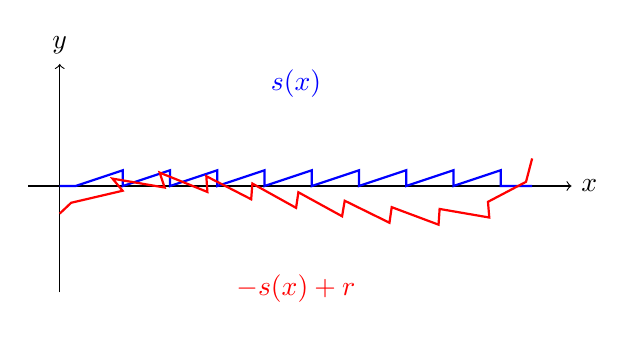
\begin{tikzpicture}[x=1cm,y=1cm]
  \draw[->] (-.4,0) -- (6.5,0) node[right] {$x$};
  \draw[->] (0,-1.35) -- (0,1.55) node[above] {$y$};
  \draw[blue,thick,decorate,
    decoration={saw,segment length=6mm,amplitude=2mm,pre length=2mm,post length=2mm}]
    (0,0) -- (6,0);
  \draw[red,thick,decorate,
    decoration={saw,segment length=6mm,amplitude=2mm,mirror,raise=1mm,pre length=2mm,post length=2mm}]
    (0,-.35) .. controls (1.4,1.15) and (4.6,-1.1) .. (6,.35);
  \node[blue,above] at (3,1) {$s(x)$};
  \node[red,below] at (3,-1) {$-s(x)+r$};
\end{tikzpicture}
\end{document}
